\chapter{Institutional Background and Literature Review}\label{ch:background}

\section{Program Structure and Premium Components}\label{sec:structure}

MAFRA delegates program management to the Agricultural Policy Insurance \& Finance Service (APFS). NH Nonghyup Property \& Casualty Insurance (NH), the single operator, sells contracts through local agricultural cooperatives, services them, and pays indemnities. Figure~\ref{fig:organization} summarizes the payments and risk transfers among these parties.

\begin{figure}[htbp]
\centering
\IfFileExists{organization.tex}{%
  \adjustbox{max width=\textwidth}{\input{organization}}%
}{%
  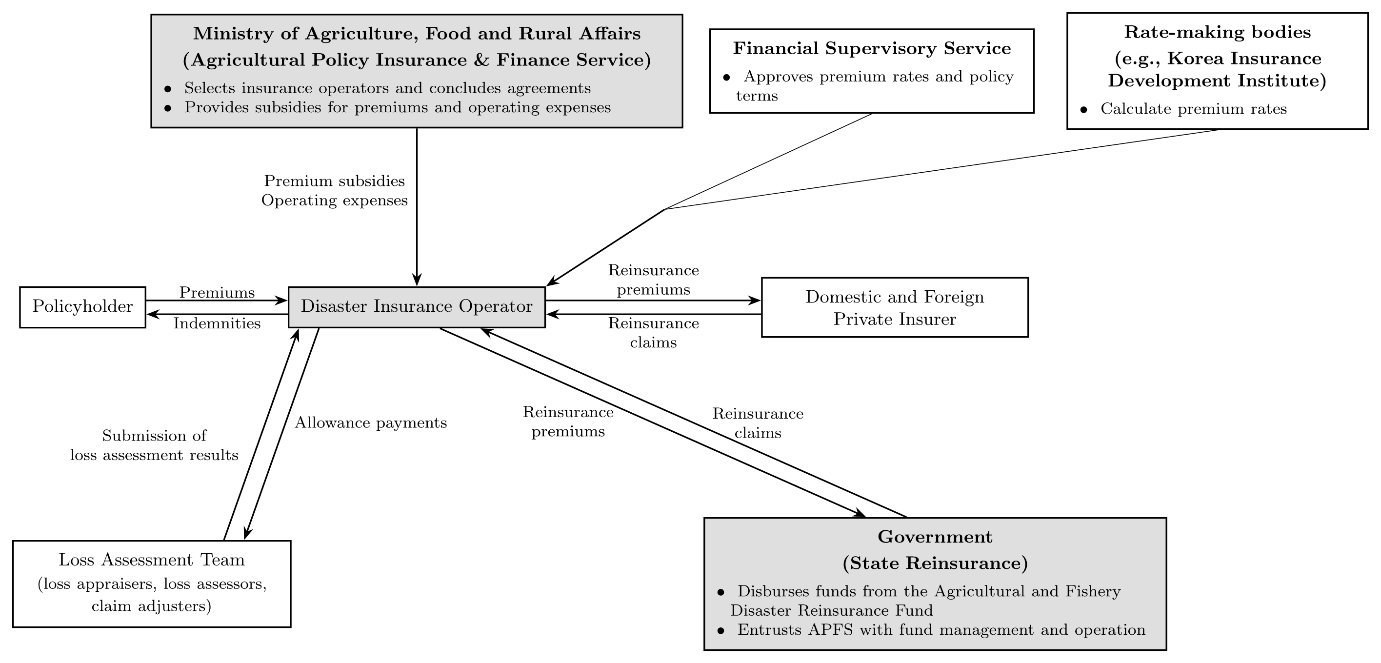
\includegraphics[width=\textwidth]{figures/fig1_organization_fallback.png}%
}
\caption{Organizational Structure of Crop Disaster Insurance in South Korea}\label{fig:organization}
\notes{Arrows indicate payments and the submission of loss assessment results; dashed lines indicate the verification and approval of premium rates and policy terms. Local agricultural cooperatives, which sell contracts on behalf of the operator, are not shown. Adapted from \citet{mafra2025,mafra2026}.}
\end{figure}

NH shares its risk with private reinsurers and with the Agricultural and Fishery Disaster Reinsurance Fund. In 2024, the first-stage shares of the main program's profit-and-loss-sharing arrangement were 10 percent for NH, 40 percent for private reinsurers, and 50 percent for the state \citep[p.~274]{mafra2025}. Additional non-proportional provisions change these shares at higher loss levels, so the first-stage shares do not describe every layer of loss.

The gross premium has two components. The pure premium covers the insured risk and loss-investigation expenses, whereas the premium loading covers specified operating expenses, including delegated selling costs. Under the 2026 rules, the government pays part of the pure premium and all of the loading \citep{mafra2026}. The subsidy rate in equation~\eqref{eq:demand} therefore refers to the pure premium, and the public share of the gross premium is higher than that rate suggests.

\section{Expansion, Enrollment, and Financing}\label{sec:expansion}

The program began with apples and pears in 2001 and covered 78 crops and 94 products in 2026 \citep{mafra2026}. Pilot introduction, expansion of sales regions, and main-program status can fall in different years. The national comparison uses the last pre-pilot year as its reference and ten crop-specific target years beginning with the coded expansion year (Table~\ref{tab:timing}). These milestones distinguish program availability from actual enrollment.

Enrollment, defined as insured area divided by eligible area, rose from 12.5 percent in 2009 to 54.2 percent in 2024 (Figure~\ref{fig:enrollment}). Because eligible area grows whenever crops or regions are added, the national rate reflects program scope as well as take-up. The loss ratio compares claims with premiums for the insurance portfolio; it measures neither income losses of individual farms nor NH's company-wide profitability after reinsurance.

Figure~\ref{fig:premiumshares} shows how the pure premium is financed. In 2024, local governments paid 39.7 percent and policyholders 12.6 percent, leaving 47.7 percent to the central government. Central and local pure-premium support totaled KRW 996.9 billion across 676,226 insured hectares, or approximately KRW 1.47 million per insured hectare \citep{apfs}. This expenditure measure excludes the publicly financed loading; individual transfers vary with insured value, rated risk, and coverage.

\begin{figure}[htbp]
\centering
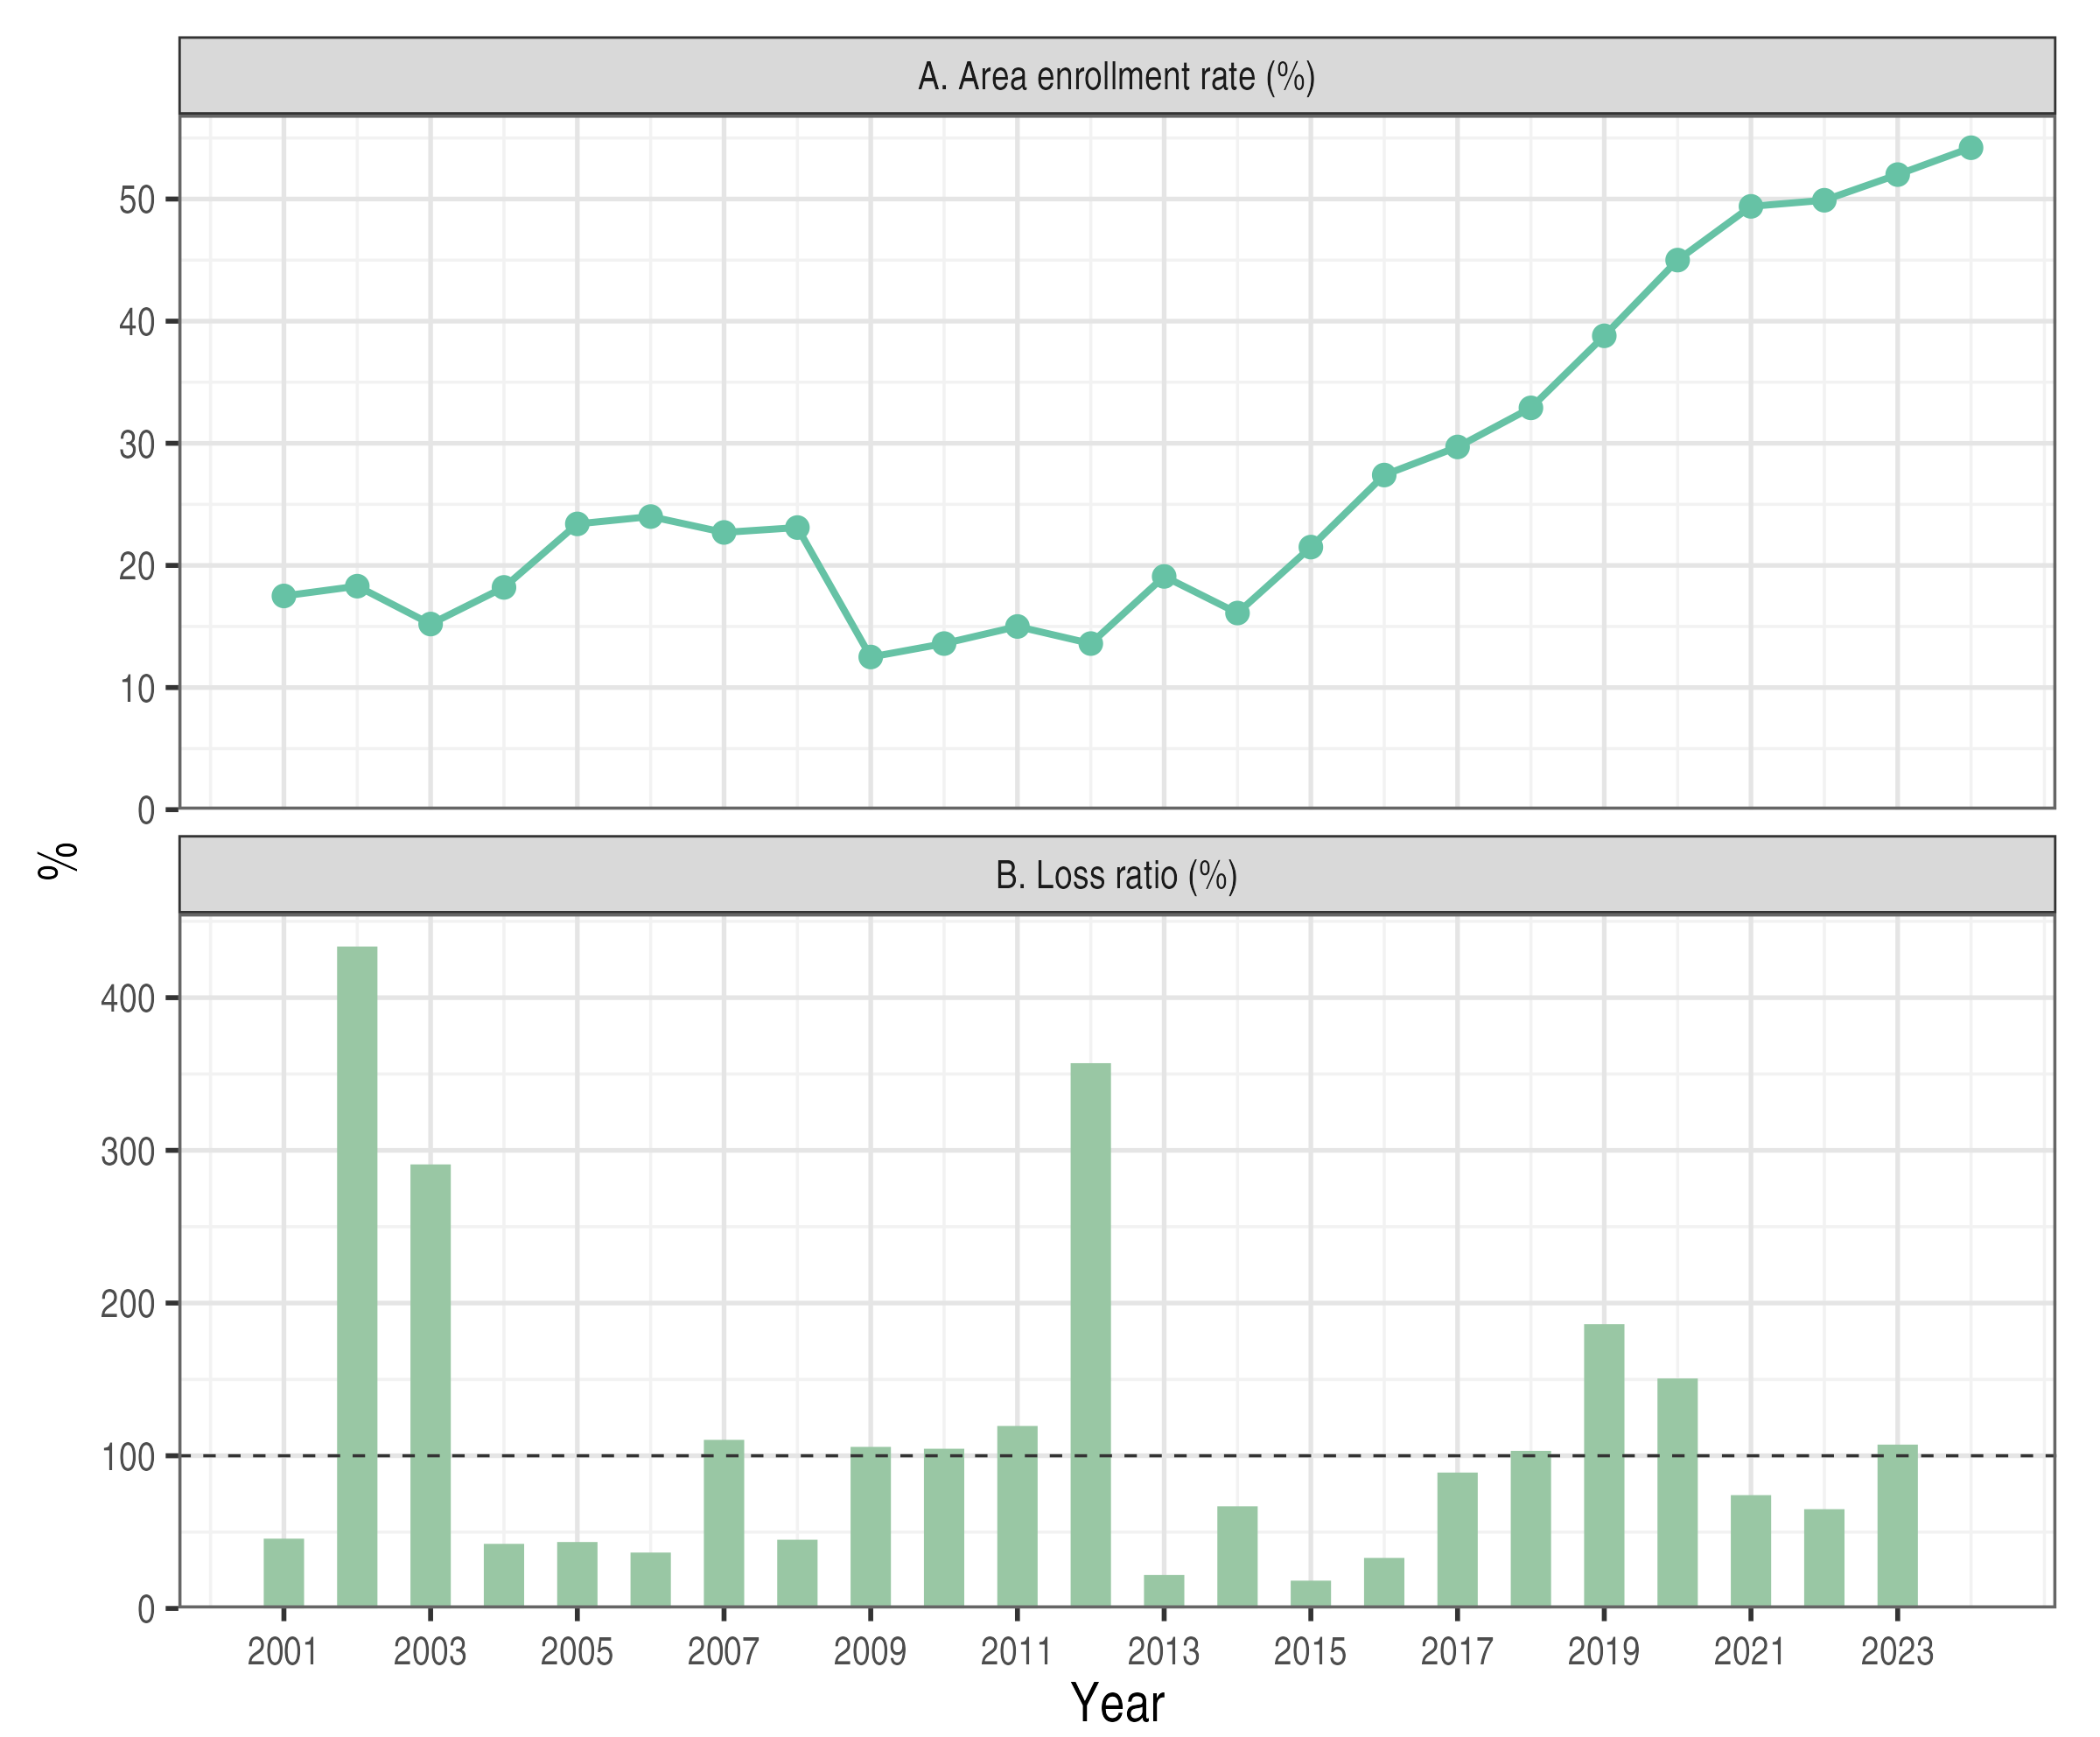
\includegraphics[width=5.0in]{figures/fig2_enrollment_loss_ratio.png}
\caption{National Enrollment Rate and Loss Ratio, 2001-2024}\label{fig:enrollment}
\notes{Enrollment is insured area divided by eligible area. The loss ratio is indemnities divided by premium net of refunds through 2011 and by risk premium from 2012; it is shown through 2023. The horizontal line marks 100 percent. Data from \citet{apfs}.}
\end{figure}

Enrollment also differs sharply across crops (Table~\ref{tab:enrollment}). In 2023, 89.0 percent of eligible apple area and 61.0 percent of eligible rice area were insured, compared with 7.1 percent for sweet potato and 5.4 percent for corn. For the seven annual crops analyzed in Chapter~\ref{ch:results}, the availability of insurance therefore translated into very different degrees of actual coverage.

\begin{figure}[htbp]
\centering
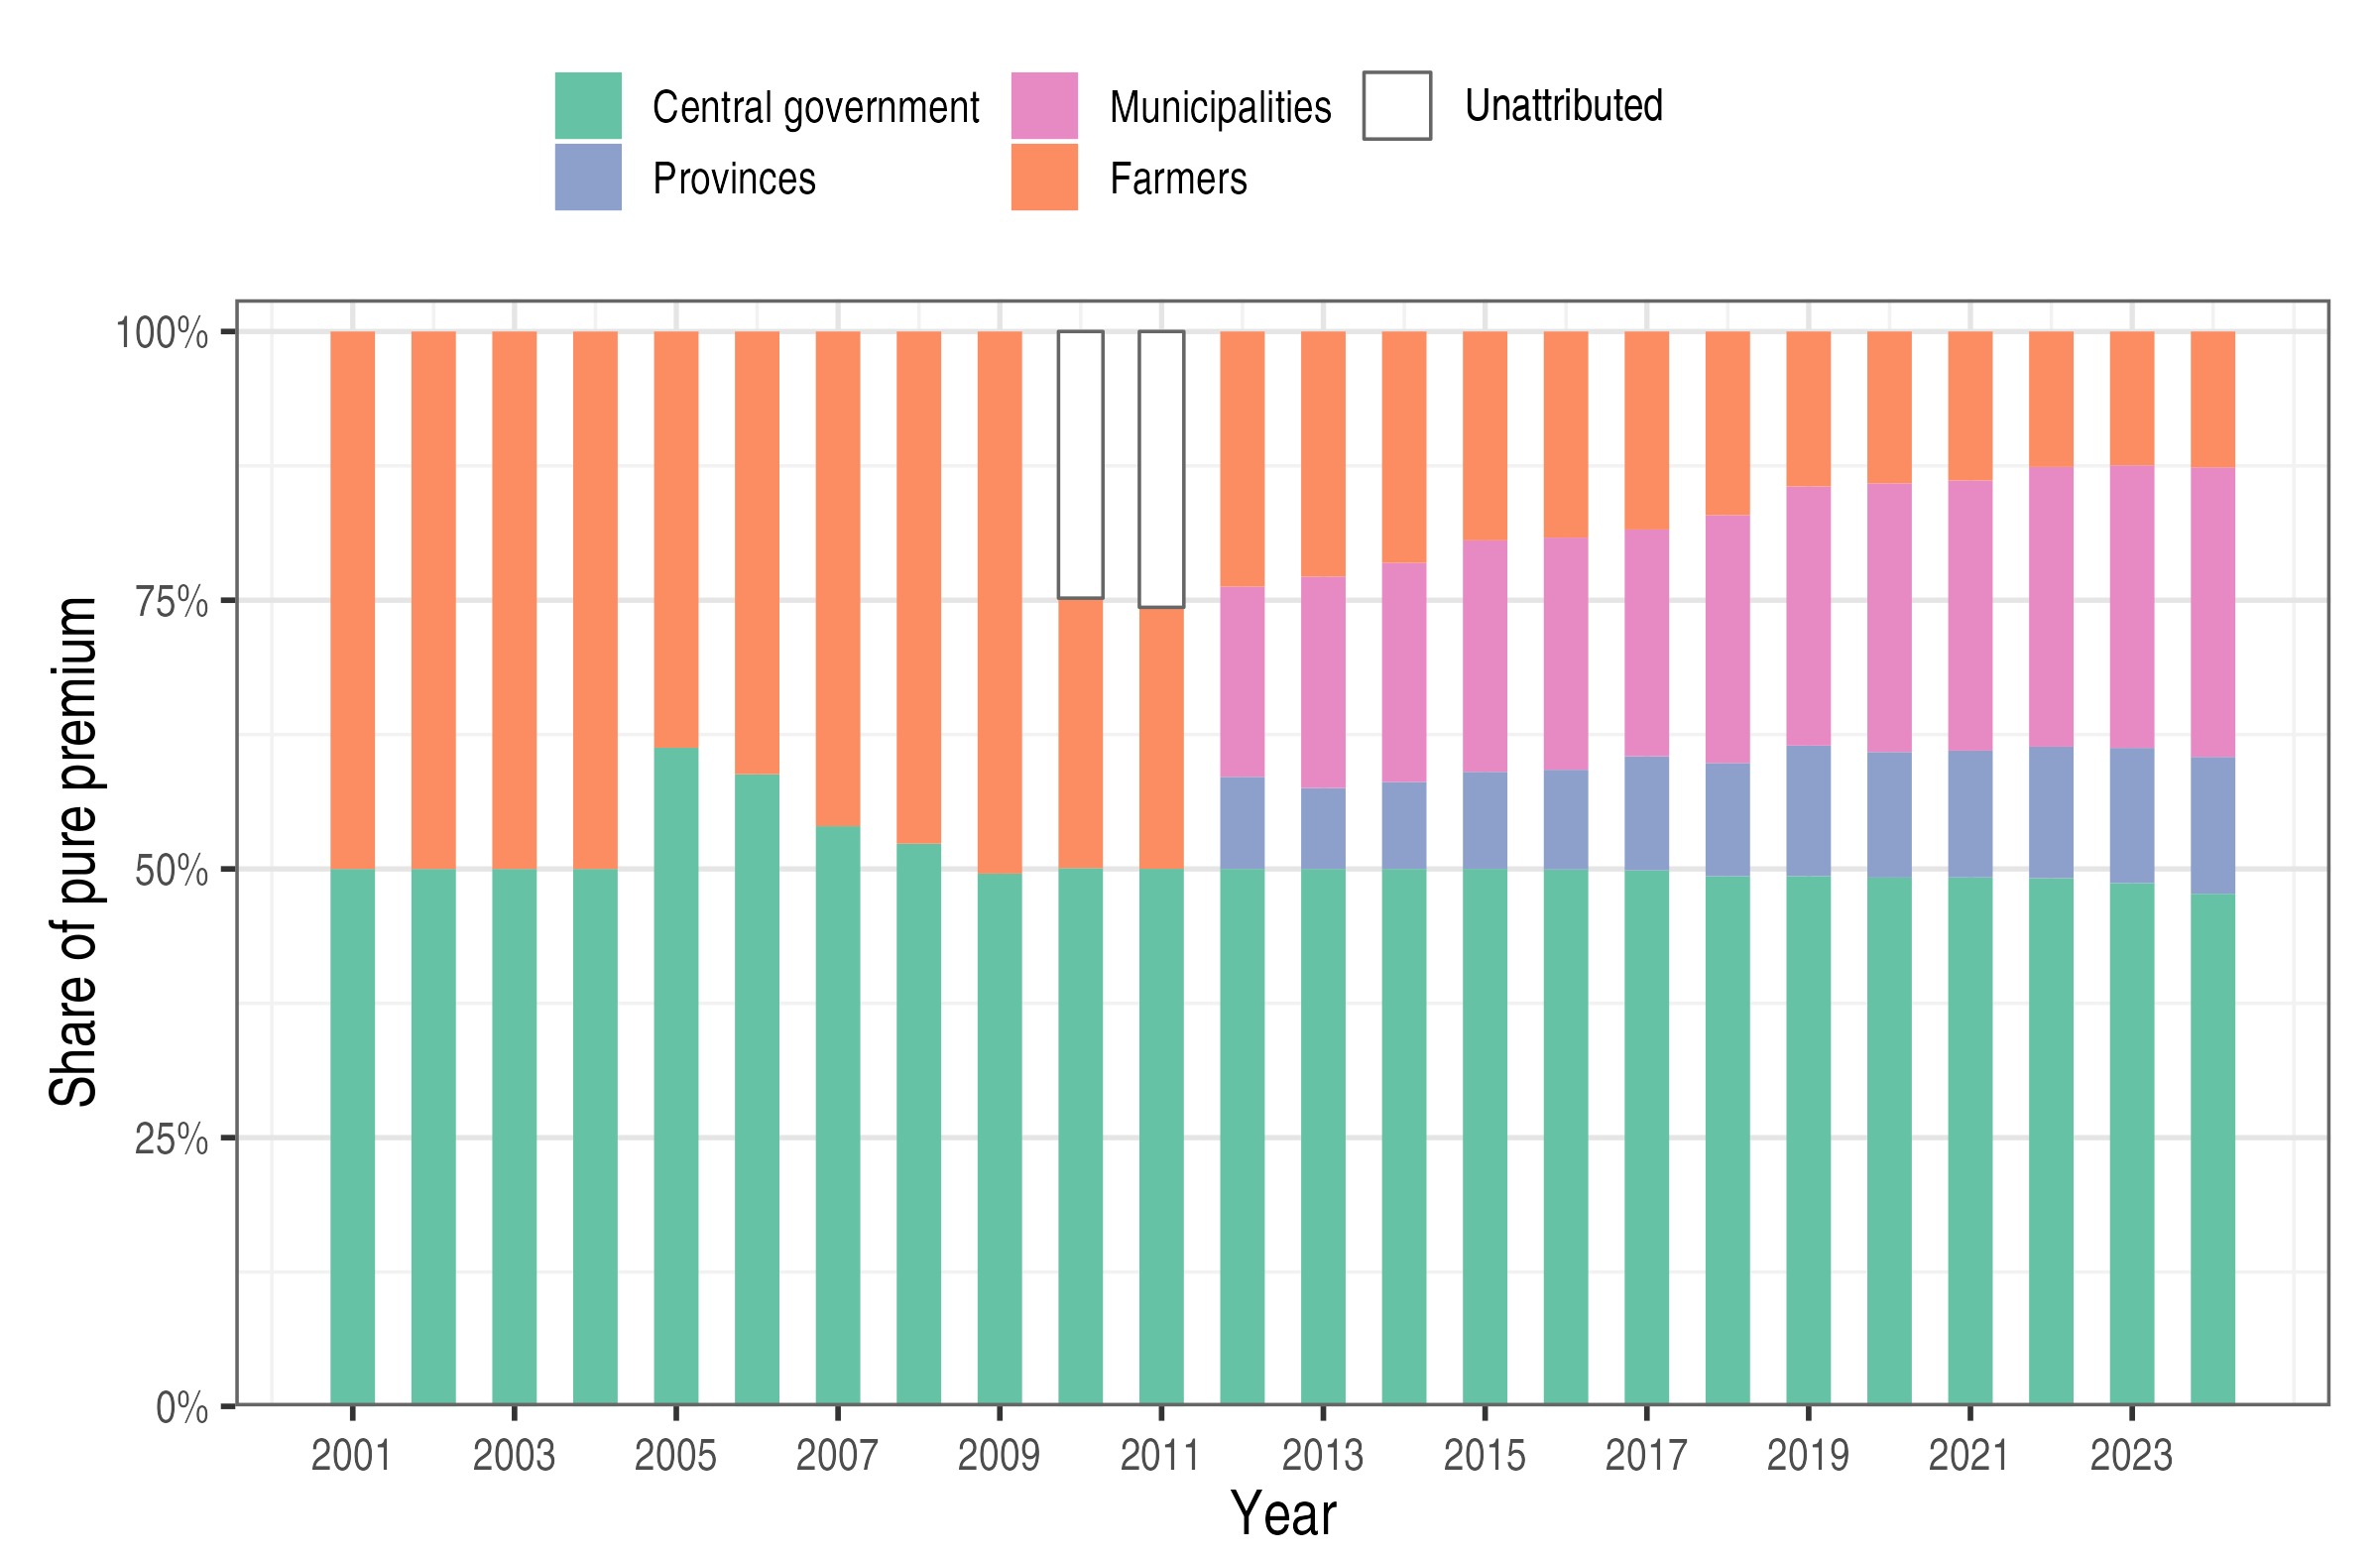
\includegraphics[width=5.4in]{figures/fig3_pure_premium_shares.png}
\caption{Shares of the Pure Premium by Payer, 2001-2024}\label{fig:premiumshares}
\notes{Shares of the reported pure-premium total. Unattributed segments in 2010-2011 are the difference between that total and the identified payer components. The publicly financed loading is excluded. Data from \citet{apfs}.}
\end{figure}

\begin{table}[htbp]
\centering
\caption{Enrollment and Loss Ratios for Selected Crops, 2023}\label{tab:enrollment}
\begin{tabular*}{\textwidth}{@{\extracolsep{\fill}}lcccc}
\toprule
Crop & Eligible area (ha) & Insured area (ha) & Enrollment (\%) & Loss ratio (\%) \\
\midrule
\multicolumn{5}{@{}l}{\textit{Panel A. Rice and major fruits}} \\
Rice          & 725,882 & 443,136 & 61.0 & 103.5 \\
Apple         & 24,945  & 22,209  & 89.0 & 116.1 \\
Pear          & 10,078  & 7,683   & 76.2 & 60.5  \\[4pt]
\multicolumn{5}{@{}l}{\textit{Panel B. Seven annual crops}} \\
Soybean       & 55,326  & 28,649  & 51.8 & 158.9 \\
Onion         & 17,128  & 6,811   & 39.8 & 73.1  \\
Garlic        & 21,110  & 5,936   & 28.1 & 119.0 \\
Red pepper    & 26,126  & 8,522   & 32.6 & 141.7 \\
Spring potato & 3,793   & 727     & 19.2 & 247.8 \\
Sweet potato  & 18,389  & 1,300   & 7.1  & 195.5 \\
Corn          & 14,073  & 764     & 5.4  & 129.2 \\
\bottomrule
\end{tabular*}
\notes{Eligible area can differ from national cultivated area because it depends on each product's sales regions. The loss ratio is indemnities divided by risk premium. Data from \citet{apfs}; author's calculations.}
\end{table}

\section{Related Literature}\label{sec:literature}

Asymmetric information and correlated losses motivate distinct forms of public involvement. Nelson and Loehman \citeyearpar{nelson1987} analyze agricultural insurance contracts under information problems, and \citet{just1999} distinguish actuarial incentives from asymmetric information in participation. Lee and Jung \citeyearpar{leejung2014} examine adverse selection and moral hazard in Korea. Miranda and Glauber \citeyearpar{miranda1997} emphasize systemic risk and reinsurance capacity. \citet{jia2025} show that the appropriate public role depends on loss correlation and relative risk-bearing efficiency. Kang and Chung \citeyearpar{kang2017} examine the implications of Korea's risk-group reinsurance arrangement for the state fund.

Insurance demand reflects differences in risk exposure, financial resources, and the value farmers place on protection, so a common subsidy rate need not generate uniform participation \citep{hazell2017}. Expected disaster relief may also reduce insurance demand through charity hazard \citep{coate1995,raschky2007}. \citet{lusk2017} distinguishes distributional transfers from economic costs. These perspectives separate access, redistribution, and welfare as questions for policy evaluation.

Studies of production responses address different margins. \citet{goodwin2004} and \citet{yu2018} examine acreage responses to U.S. crop insurance and premium subsidies. \citet{han2014} studies production and price effects in Korea, Nam and Ahn \citeyearpar{nam2022} examine input use and farm income, and Lee and Kim \citeyearpar{leekim2026} study insured fruit farms. The present analysis combines an assessment of support instruments with comparisons of aggregate area, yield, and production. Availability-based contrasts differ from estimates of responses among enrolled farms.

Methodologically, timing-specific comparisons avoid using already-exposed units as controls \citep{callaway2021}, but their validity still depends on whether the comparison units trace the untreated path of the treated units. \citet{roth2022} shows that passing a pretrend test does not establish parallel trends and that conditioning on such tests can distort inference. With few treated clusters, cluster-robust and bootstrap inference can be unreliable \citep{cameron2008,mackinnonwebb2018,mackinnon2023,webb2023}, a concern that applies directly to seven treated crops.
